\documentclass{article}
\usepackage{pgfplots}
\usepgfplotslibrary{fillbetween}

\title{ AP Calculus AB Take-Home Final }
\begin{document}
\author{
	Duncan Freeman
}

\maketitle

% TODO: Make a .cls for 'Take-home-final' that removes the subsection numbers, and puts \hline and \vspace{5mm} after sections.
% Also make boxing answers a thing ala https://tex.stackexchange.com/questions/20575/attractive-boxed-equations#20582

\section{}
\hline
\vspace{5mm}
\begin{center}
	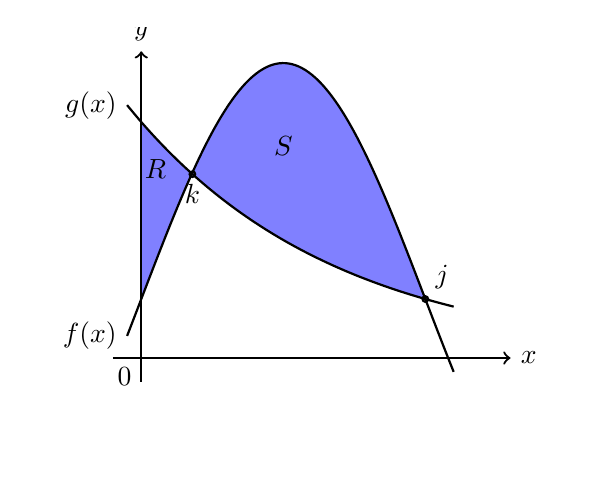
\begin{tikzpicture}
		\begin{axis}[thick,smooth,no markers, hide axis, ymin=-0.5, ymax=1.4, xmin=-0.4, xmax=1.5]
			\addplot+[name path=A,black, samples=100, domain=-0.05:1.1] {0.25 + sin((\x * pi) r)} node[left, pos=0] {$f(x)$};
			\addplot+[name path=B,black, domain=-0.05:1.1] {4^(-x)} node[left, pos=0] {$g(x)$};
			\addplot[blue!50] fill between[of=A and B, soft clip={domain=0:1}];
			\draw[arrows=->, thick] (axis cs:-0.1,0) -- (axis cs:1.3,0) node[right] {$x$};
			\draw[arrows=->, thick] (axis cs:0,-0.1) -- (axis cs:0,1.3) node[above] {$y$};
			\draw[thick] (axis cs:0.180, 0.779) circle(1pt) node[below] {$k$};
			\draw[thick] (axis cs:1, 0.25) circle(1pt) node[above right] {$j$};
			\node at (axis cs:0.5, 0.9) {$S$};
			\node at (axis cs:0.05, 0.8) {$R$};
			\node[below left] at (axis cs:0, 0) {$0$};
		\end{axis} 
	\end{tikzpicture}
\end{center}

\begin{center}
	\noindent
	$f(x) = \frac{1}{4} + \sin{\pi x}, \enspace g(x) = 4^{-x}$ \\
\end{center}

\subsection{Part A}
First, we find the first intersection of $f(x)$ and $g(x)$. We'll call the $x$ value of the intersection $k$. We can then use a calculator approximate the integration of the difference between $g(x)$ and $f(x)$ from $0$ until $k$ to obtain the area $R$.
\[ R = \int_{0}^{k} [g(x) - f(x)]dx \approx 0.064 \]

\subsection{Part B}
Next, we can find the second intersection of $f(x)$ and $g(x)$ (which we will call $j$. We can then integrate similarly to get the area; Note that we reverse the order of $g(x)$ and $f(x)$ because $f(x)$ has a higher value of $y$.
\[	S = \int_{k}^{j} [f(x) - g(x)]dx \approx 0.410 \]

\subsection{Part C}
To revolve $S$ around the horizontal line $y = -1$, we have to adjust $f(x)$ and $g(x)$ by $+1$, and then shroud them in the circle area equation $\pi r^2$, finally integrating the resulting difference between $k$ and $j$ to obtain volume.
\[ S_{\text{vol}} = \pi\!\int_{k}^{j} [(f(x)+1)^2 - (g(x)+1)^2]\,dx \approx 4.56 \]

Sorry there's no graphic for the revolve, it's \textit{hard.}


\section{}
\hline
\vspace{5mm}
\[ f(0) = 2, \enspace f'(0) = -4, \enspace f''(0) = 3 \]

\subsection{Part A}
\[ g(x) = e^{ax} + f(x) \]
First, we need to know the derivatives of $g(x)$, so we evaluate them as such:
\[ \frac{d}{dx} g(x) = g'(x) = ae^{ax} + f'(x) \]
\[ \frac{d}{dx} g'(x) = g''(x) = e^{ax}a^2 + f''(x) \]
Next, we can evaluate the derivatives of $g(x)$ in line with the pre-defined derivatives of $f(x)$ like so:
\[ g'(0) = ae^{a(0)} + f'(0) = ae^0 - 4 = a - 4 \]
\[ g''(0) = e^{a(0)}a^2 + f''(0) = a^2e^0 + 3 = a^2 + 3 \]
\subsection{Part B}
\[ h(x) = \cos{(kx)}f(x) \]
First, we derive $h(x)$:
\[ \frac{d}{dx} h(x) = h'(x) = -k\sin{(kx)}f(x) + \cos{(kx)}f'(x) \]
This gave us the slope ($h'(0)$), but we still need to find the y value of $h(0)$ and the slope at $h'(0)$
\[ y = h(0) = \cos{[k(0)]}f(0) = \cos{(0)}(2) = (1)(2) = 2 \]
\[ m = h'(0) = -k\sin{(k0)}f(x) + \cos{(k0)}f'(0) = 0 + \cos{(1)}(-4) = -4 \]
We can finally find the tangent equation:
\[ y - 2 = -4 ( x - 0 ) \]


\end{document}

